\section{Results}
\label{sec:results}

\subsection{The frozen comparison}
\label{sec:results-frozen}

With the encoder frozen, the two self-training methods reach about twice the TPR of the
source-only baseline (Table~\ref{tab:frozen}, Appendix~\ref{sec:frozen-comparison}): AdaMatch $\dFrozenAda{}$ and FreeMatch
$\dFrozenFm{}$ against $\dFrozenBase{}$, paired differences $\dFrozenAdaDiff{}$
$[\dFrozenAdaLo{}, \dFrozenAdaHi{}]$ and $\dFrozenFmDiff{}$ $[\dFrozenFmLo{}, \dFrozenFmHi{}]$
under the class-conditional paired bootstrap. CORAL sits at $\dFrozenCoral{}$, a difference
from the baseline that excludes zero only at the margin, and the DANN development run scored
exactly what Baseline A scores on the same fold and pool. These arms were not trained under
identical conditions: the feature-space arms ran without augmentation at full precision and the
image-space arms with weak augmentation at half precision (Appendix~\ref{sec:augprec}).
Unfreezing raised FreeMatch's TPR by $\dLpDiff{}$ $[\dLpLo{}, \dLpHi{}]$ (fold-aware paired
bootstrap; Table~\ref{tab:contrasts6}, last row); the frozen and unfrozen FreeMatch runs share
every training setting except the encoder and the 1500 further steps of training, and a
\restartControlStepsNs{}-step frozen continuation tracked the frozen run
(Appendix~\ref{sec:appendix-restart}). It is the only frozen-against-unfrozen contrast we
report; Section~\ref{sec:results-ablation} uses it, with the frozen head's own score, to split
FreeMatch's contrast against the control into the parts gained before and after unfreezing.
The unfrozen arms do not reproduce the
frozen separation between the method families (Section~\ref{sec:results-ablation}), so we treat
that separation as a property of the frozen protocol as we ran it.

\subsection{The main table}
\label{sec:results-main}

Table~\ref{tab:main2} gives the unfrozen arms on folds 1--4. Baseline A and the $\lambda=0$
control both reach $\dFmBaseline{}$, BNM $\dFmBnm{}$, and FreeMatch, DANN and CORAL
$\dFmFreeMatch{}$, $\dFmDann{}$ and $\dFmCoral{}$. Their spreads across folds differ
($\dSdFreeMatch{}$, $\dSdDann{}$ and $\dSdCoral{}$), and at four folds none is well
determined. Baseline A's row is its folds 1--4 mean; its five-fold mean belongs to
Table~\ref{tab:frozen}, and fold 0 enters no confirmatory number.

% GENERATED FILE -- do not edit by hand.
% Rebuild:  python make_all.py (generator: make_main_tables_v2.py)
% Table 2 (rewrite v1): the main table at two decimals. _common.fold_mean on pool D1.
\begin{table}[tbp]
\centering
\caption{\textbf{Main results.} TPR at FPR${}=10^{-3}$ on the cleaned test pool, mean and sample sd over the confirmatory folds 1--4; each arm is read at its final budget except BNM, whose rule gave 1000 steps and which is read at 4000, where its control is read (Appendix~\ref{sec:budget-detail}). Per-fold and four-decimal values: Appendix~\ref{app:perfold}.}
\label{tab:main2}
\footnotesize
\setlength{\tabcolsep}{4pt}
\begin{tabular}{lrrrl}
\toprule
Arm & TPR@$10^{-3}$ & sd & Read at & Encoder \\
\midrule
Baseline A & $0.18$ & $0.03$ & 8000 & frozen \\
$\lambda=0$ control & $0.18$ & $0.03$ & 4000 & unfrozen \\
BNM & $0.40$ & $0.04$ & 4000 & unfrozen \\
FreeMatch & $0.52$ & $0.07$ & 1500 & unfrozen \\
DANN & $0.50$ & $0.17$ & 4000 & unfrozen \\
CORAL & $0.52$ & $0.08$ & 2000 & unfrozen \\
DANN, sensitivity readout & $0.55$ & $0.11$ & 2000 & unfrozen \\
\bottomrule
\end{tabular}
\end{table}


\subsection{What a target signal buys}
\label{sec:results-ablation}

Table~\ref{tab:contrasts6} and Figure~\ref{fig:forest} give the paired contrasts. The three
contrasts against the control, registered before the control ran, are large. DANN $-$ $\lambda=0$ at 4000/4000 is
$\dCtDannLam{}$ $[\dCtDannLamLo{}, \dCtDannLamHi{}]$, CORAL $-$ $\lambda=0$ at 2000/4000 is
$\dCtCoralLamP{}$ $[\dCtCoralLamPLo{}, \dCtCoralLamPHi{}]$, and FreeMatch $-$ $\lambda=0$ at
1500/4000 is $\dCtFmLamP{}$ $[\dCtFmLamPLo{}, \dCtFmLamPHi{}]$; the control starts from
DANN's head, so only the DANN row is a matched contrast, and for CORAL and FreeMatch, which start
from their own heads, it is a method-neutral baseline. Each interval excludes zero,
all four folds agree in sign, and every lower bound lies well above the one-positive step of
the metric. DANN $-$ $\lambda=0$, the fully controlled pair (Section~\ref{sec:arms}), has the
widest interval. Read at the same step as the control, as sensitivity readouts declared with these contrasts,
CORAL gives $\dCtCoralLamM{}$ $[\dCtCoralLamMLo{}, \dCtCoralLamMHi{}]$ at 2000/2000 and FreeMatch
$\dCtFmLamM{}$ $[\dCtFmLamMLo{}, \dCtFmLamMHi{}]$ at 1500/1500; these matched forms remove the
budget difference and leave the other confounds in place (Section~\ref{sec:arms}). BNM,
which was not among the contrasts registered with the control, shares DANN's head but differs
from it in how its adaptation weight was tuned and in batch order (Section~\ref{sec:arms}), and
gives
$\dCtBnmLam{}$ $[\dCtBnmLamLo{}, \dCtBnmLamHi{}]$ at 4000/4000, again with all four folds
agreeing. With a 1:10 target whose batches are drawn
without the labels, DANN and BNM keep a detectable gain over the control, and for CORAL and
FreeMatch we cannot detect one (Section~\ref{sec:results-dilute}).

The
FreeMatch contrast spans two stages of training with a target signal: the unfrozen arm starts
from its frozen-comparison head, which already reaches \rwFiveFmStart{} on these folds, so
\rwFiveFmFrozenPart{} of its $\dCtFmLamP{}$ came with the encoder frozen and
\rwFiveFmUnfrozenPart{} after unfreezing. CORAL's frozen head starts at \rwFiveCoralStart{},
a little above the control's $\dFmLambda{}$. DANN, BNM and the control start from the same head, so
DANN $-$ $\lambda = 0$ and BNM $-$ $\lambda = 0$ each measure a single stage of training; of
the two, only DANN $-$ $\lambda = 0$ differs from the control in nothing but its adaptation
weight (Section~\ref{sec:arms}). The closest prior work finds a gain of the same
kind at the same operating point: Wasserstein alignment took their encoder from 0.0 to 0.241
in TPR at FPR${}=0.1\%$~\citep{parul2024}, on a different survey and test set.

Without a target signal, unfreezing buys nothing we can detect: $\lambda=0$ $-$ Baseline A is
$\dCtLamBase{}$ $[\dCtLamBaseLo{}, \dCtLamBaseHi{}]$. The two arms also differ in augmentation
(Baseline A trains on cached, unaugmented features), training precision, compute venue, code
path and budget, so this row does not isolate unfreezing.

Our starting point is weak. Baseline A and the $\lambda=0$ control reach a TPR of
$\dFmBaseline{}$, and at the benchmark's operating point of 24\% purity Baseline A recovers
$\dLrBaseline{}$\% of the completeness of Lines et al.'s simulation-only model. Their model
differs from ours in its simulations (one of its two simulation sets uses real HST source
galaxies, the other synthetic sources made of one to four S\'ersic components; ours are single-component or
bulge-plus-disk fits), its
negatives and its fine-tuning, and we cannot say which difference accounts for the gap. The
adaptation arms reach $\dLrDaMin{}$--$\dLrDaMax{}$\% of that completeness. What we measure is
therefore a gain over our own simulation-only baseline; whether adaptation would add anything
to a stronger simulation-only model is untested.

The control is one source-only fine-tune, not a tuned best one. The gain does not rest on this
control alone: Baseline A, which never unfreezes, also reaches $\dFmBaseline{}$, and with the
encoder frozen FreeMatch already gains $\dFrozenFmDiff{}$ over the source-only baseline
(Section~\ref{sec:results-frozen}). On the development fold the control ends
below the frozen linear-probe head it started from, at $\dFzLambdaLast{}$ against $\dFzInit{}$
(Figure~\ref{fig:fold0}), the feature distortion that motivates fitting a linear probe before
fine-tuning~\citep{kumar2022lpft}, and a Euclid Q1 transformer retrained on real labels showed a
related drop when fully unfrozen~\citep{astrovink}. That observation rests on one fold, and our statement that
a target signal is needed is relative to this control.

Between objectives, one comparison excludes zero: BNM $-$ CORAL at 2000/2000 is
$\dCtBnmCoral{}$ $[\dCtBnmCoralLo{}, \dCtBnmCoralHi{}]$, with all four folds agreeing. We did
not pre-register it, and it is one of the \contrastCount{} $t$-intervals of the main design, reported
without multiplicity correction. BNM $-$ DANN and BNM $-$
FreeMatch admit zero, and so do DANN $-$ CORAL and DANN $-$ FreeMatch at their declared budgets
and DANN $-$ CORAL at 2000/2000. Section~\ref{sec:resolution} discusses how far these
comparisons can rank the arms.

% GENERATED FILE -- do not edit by hand.
% Rebuild:  python make_all.py (generator: make_dilute10_tables.py)
% Table 2 (paper v6): tables/T3v2_contrasts.tex unchanged, plus the 1:10 block from runs/dilute10_analysis/results.json (G primary).
\begin{table}[tbp]
\centering
\caption{\textbf{Paired contrasts} in TPR at FPR${}=10^{-3}$, folds 1--4, cleaned pool: mean difference, paired $t$-interval (df${}=3$), and the number of folds agreeing in sign. $^{\dagger}$Registered with the $\lambda=0$ control, before it ran but after the adaptation arms' results were known (Section~\ref{sec:prereg}). $^{\ddagger}$Sensitivity readout declared with those contrasts. Steps give where each arm is read. $^{\S}$From the second experiment, with a 1:10 target whose batches are drawn without the labels (Section~\ref{sec:results-dilute}): the arm's diluted run against the same $\lambda=0$ control, pre-registered as that experiment's primary contrast; a bound that rounds to zero at two decimals is shown at three, and the matched-step forms and the balanced $-$ diluted contrasts are in Table~\ref{tab:dl-contrasts4}. Four-decimal values: Tables~\ref{tab:contrasts4} and~\ref{tab:dl-contrasts4}.}
\label{tab:contrasts6}
\footnotesize
\setlength{\tabcolsep}{4pt}
\begin{tabular}{llrrc}
\toprule
Contrast & Steps & $\Delta$ & 95\% CI & Signs \\
\midrule
\multicolumn{5}{l}{\textit{Frozen against unfrozen, no target signal}} \\
$\lambda=0$ $-$ Baseline A$^{\dagger}$ & 4000 / 8000 & $0.00$ & $[-0.09, +0.09]$ & 3/4 \\
\midrule
\multicolumn{5}{l}{\textit{A target signal against none}} \\
DANN $-$ $\lambda=0$$^{\dagger}$ & 4000 / 4000 & $+0.31$ & $[+0.06, +0.57]$ & 4/4 \\
CORAL $-$ $\lambda=0$$^{\dagger}$ & 2000 / 4000 & $+0.34$ & $[+0.19, +0.49]$ & 4/4 \\
FreeMatch $-$ $\lambda=0$$^{\dagger}$ & 1500 / 4000 & $+0.33$ & $[+0.23, +0.44]$ & 4/4 \\
CORAL $-$ $\lambda=0$$^{\ddagger}$ & 2000 / 2000 & $+0.31$ & $[+0.18, +0.43]$ & 4/4 \\
FreeMatch $-$ $\lambda=0$$^{\ddagger}$ & 1500 / 1500 & $+0.32$ & $[+0.20, +0.45]$ & 4/4 \\
BNM $-$ $\lambda=0$ & 4000 / 4000 & $+0.22$ & $[+0.14, +0.30]$ & 4/4 \\
\midrule
\multicolumn{5}{l}{\textit{A target signal against none, 1:10 target}} \\
DANN$^{\S}$ $-$ $\lambda=0$ & 4000 / 4000 & $+0.33$ & $[+0.29, +0.38]$ & 4/4 \\
BNM$^{\S}$ $-$ $\lambda=0$ & 4000 / 4000 & $+0.19$ & $[+0.003, +0.39]$ & 4/4 \\
CORAL$^{\S}$ $-$ $\lambda=0$ & 2000 / 4000 & $+0.01$ & $[-0.03, +0.05]$ & 3/4 \\
FreeMatch$^{\S}$ $-$ $\lambda=0$ & 1500 / 4000 & $+0.25$ & $[-0.004, +0.51]$ & 4/4 \\
\midrule
\multicolumn{5}{l}{\textit{Objective against objective}} \\
BNM $-$ CORAL & 2000 / 2000 & $-0.12$ & $[-0.18, -0.06]$ & 4/4 \\
BNM $-$ DANN & 4000 / 4000 & $-0.09$ & $[-0.31, +0.12]$ & 3/4 \\
BNM $-$ FreeMatch & 1500 / 1500 & $-0.13$ & $[-0.30, +0.03]$ & 4/4 \\
DANN $-$ CORAL & 4000 / 2000 & $-0.02$ & $[-0.22, +0.18]$ & 2/4 \\
DANN $-$ FreeMatch & 4000 / 1500 & $-0.02$ & $[-0.21, +0.17]$ & 2/4 \\
DANN $-$ CORAL & 2000 / 2000 & $+0.03$ & $[-0.07, +0.14]$ & 2/4 \\
\midrule
\multicolumn{5}{l}{\textit{Frozen against unfrozen, same objective (fold-aware paired bootstrap)}} \\
FreeMatch unfrozen $-$ frozen & 1500 / 8000 & $+0.10$ & $[+0.03, +0.17]$ & 4/4 \\
\bottomrule
\end{tabular}
\end{table}


\begin{figure}[t]
\centering
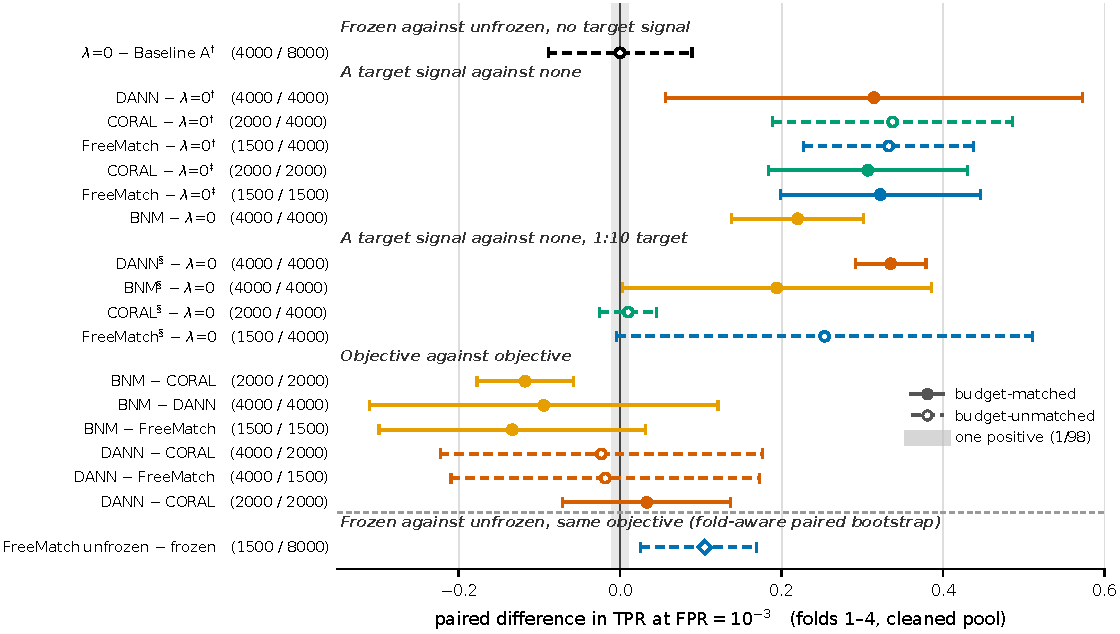
\includegraphics[width=\textwidth]{F3_forest_v6.pdf}
\caption{\textbf{The paired contrasts of Table~\ref{tab:contrasts6}.} Paired $t$-intervals on
four per-fold differences; filled markers are budget-matched, open markers are not.
$^{\dagger}$Registered with the $\lambda=0$ control, before it ran; $^{\ddagger}$sensitivity
readout declared with those contrasts; $^{\S}$from the
second experiment, with a 1:10 target whose batches are drawn without the labels, against the same control
(Section~\ref{sec:results-dilute}). The grey band is one positive ($1/98$). The last row uses
the fold-aware paired bootstrap.}
\label{fig:forest}
\end{figure}

\subsection{A 1:10 target with batches drawn without the labels}
\label{sec:results-dilute}

Table~\ref{tab:dilute} and Figure~\ref{fig:dilute} give the second experiment
(Section~\ref{sec:dilute-methods}). Its four pre-registered branch sentences follow. In these
sentences, as in the pre-registration, ``drawn without the labels'' refers to the target
batches; the pool itself is built from catalogue lenses (Section~\ref{sec:labels}).

\begin{quote}
With a 1:10 target drawn without the labels, DANN still raises TPR@$10^{-3}$ over the control
by $\dlGDannFour{}$ $[\dlGDannLoFour{}, \dlGDannHiFour{}]$, and we detect no loss against the
balanced target ($\dlDDannFour{}$ $[\dlDDannLoFour{}, \dlDDannHiFour{}]$), though the interval
admits losing up to $\dlDDannHiAbsFour{}$ of the original $\dlBalDannAbsFour{}$.

With a 1:10 target drawn without the labels, BNM still raises TPR@$10^{-3}$ over the control by
$\dlGBnmFour{}$ $[\dlGBnmLoFour{}, \dlGBnmHiFour{}]$, and we detect no loss against the balanced
target ($\dlDBnmFour{}$ $[\dlDBnmLoFour{}, \dlDBnmHiFour{}]$), though the interval admits losing
up to $\dlDBnmHiAbsFour{}$ of the original $\dlBalBnmAbsFour{}$.

We cannot detect a gain for CORAL with a 1:10 target: $\dlGCoralFour{}$
$[\dlGCoralLoFour{}, \dlGCoralHiFour{}]$.

We cannot detect a gain for FreeMatch with a 1:10 target: $\dlGFmFour{}$
$[\dlGFmLoFour{},\allowbreak\ \dlGFmHiFour{}]$.
\end{quote}

\noindent With the control read at each arm's own step, CORAL gives $\dlGmCoral{}$
$[\dlGmCoralLo{}, \dlGmCoralHi{}]$ and FreeMatch $\dlGmFm{}$ $[\dlGmFmLo{}, \dlGmFmHi{}]$, the
same branches (Table~\ref{tab:dl-contrasts4}).

The two verdicts closest to zero fall on opposite sides of it by almost nothing: BNM's interval
clears zero by $\dlGBnmLoAbsThree{}$ and FreeMatch's misses it by $\dlGFmLoAbsThree{}$, and
FreeMatch's point estimate is the larger of the two. On the original test pool FreeMatch's
interval excludes zero (Table~\ref{tab:dl-sensitivity}). We do not read the difference between
these two branches as a difference between the methods.

DANN's diluted TPR is $\dlTprDann{}$, against $\dlTprDannBal{}$ with the balanced target. Its
gain over the control on the diluted target, as a fraction of its gain on the balanced one, is
$\dlRetDann{}$, a point estimate only. Its spread across folds is far smaller: an sd of
$\dlSdDann{}$ against $\dlSdDannBal{}$. With one seed per fold, we do not read the narrower spread
as an effect of dilution. For the other arms the same ratio is $\dlRetBnm{}$ for BNM,
$\dlRetFm{}$ for FreeMatch and $\dlRetCoral{}$ for CORAL ($\dlRetmFm{}$ and $\dlRetmCoral{}$ with
the control read at the arm's own step); all are point estimates only.

In point estimates, FreeMatch's smaller diluted gain arises before unfreezing. Its diluted frozen head starts at
$\dlFmStart{}$ against $\dlFmStartBal{}$, a difference of $\dlFmFrozenDiff{}$
$[\dlFmFrozenDiffLo{}, \dlFmFrozenDiffHi{}]$ under the class-conditional paired bootstrap, while
the gain from unfreezing is similar on both targets: $\dlFmUnfrozenPart{}$ against
$\dlFmUnfrozenPartBal{}$ (Table~\ref{tab:dl-frozen}), so its unfrozen stage gains slightly more
on the diluted target than on the balanced one.

CORAL's diluted run differs from its balanced counterpart in more than the target. Its frozen
stage, retrained on the diluted target, ended with a layer-normalisation gain about
\dlCoralGainRatioWord{} times the balanced run's (norm $\dlCoralGainMin{}$--$\dlCoralGainMax{}$
against $\dlCoralGainRoneMin{}$--$\dlCoralGainRoneMax{}$; Table~\ref{tab:dl-heads}), although that
stage's own TPR barely changed ($\dlCoralFrozenDiff{}$
$[\dlCoralFrozenDiffLo{}, \dlCoralFrozenDiffHi{}]$). The unfrozen stage therefore started from
features of norm $\dlCoralFeatStartMin{}$--$\dlCoralFeatStartMax{}$
(Table~\ref{tab:dl-bookkeeping}), which stayed above the guard's threshold of
$\dlCoralCeiling{}$ throughout (minimum $\dlCoralFeatMin{}$), and its ranking quality fell
overall: AUROC $\dlAurocCoral{}$, below its frozen head's $\dlCoralFrozenAuroc{}$
(Table~\ref{tab:dl-frozen}) and the control's $\dlLamAuroc{}$. We cannot tell whether CORAL's diluted run shows no detectable gain
because of the diluted target acting during its unfrozen stage or because of the much larger
head its frozen stage produced on that target.

BNM's predicted-positive fraction on the diluted target batches stayed between
$\dlBnmPpMin{}$ and $\dlBnmPpMax{}$ at every logged step, $\dlBnmPpMean{}$ averaged over every
logged step of the four folds (every \dlBnmPpEvery{} steps, \dlBnmPpN{} per fold), below the
batches' true lens fraction of $\dlBnmLensFrac{}$, rather than drifting upward as we predicted.

We wrote \dlNPredWord{} predictions before any run (Table~\ref{tab:dl-predictions}) and score
them as written. Most failed. We expected DANN's gain to degrade, probably to an interval that
includes zero, and it lost nothing we can detect; we expected CORAL to lose less than DANN,
BNM to lose the most in relative terms, and FreeMatch to lose less than BNM and keep a
detectable gain, and none of these held. The parts that held: CORAL, BNM and
FreeMatch all degraded in point estimate, and FreeMatch's head start shrank. One component,
which our scoring reads as BNM's predicted-positive fraction exceeding $\dlBnmPpThreshold{}$ at
any logged step, holds under that reading, but that reading takes a maximum over \dlBnmPpN{} single-batch
values and would be met by batch noise alone, so we do not count it as support.

The diluted pool is still built from catalogued lenses, and it is far denser in lenses than the
sky (Section~\ref{sec:limitations}).

% GENERATED FILE -- do not edit by hand.
% Rebuild:  python make_all.py (generator: make_dilute10_tables.py)
% Main-text table of the 1:10 experiment. runs/dilute10_analysis/results.json (per_arm, G primary, D, verdicts).
\begin{table}[tbp]
\centering
\caption{\textbf{The 1:10 target, with batches drawn without the labels.} Per arm, folds 1--4, cleaned pool: the diluted run's TPR at FPR${}=10^{-3}$ (mean and sample sd) at the arm's read-off step; $G$, diluted $-$ $\lambda=0$, with the control read at 4000, the primary contrast; $D$, balanced $-$ diluted at the same read-off, secondary and without a verdict; and the pre-registered branch. Paired $t$-intervals (df${}=3$); Signs counts the folds agreeing with $G$'s sign. A bound that rounds to zero at two decimals is shown at three. The $\lambda=0$ control ($\dlLamTpr{}$) is shared with Table~\ref{tab:main2}. Matched-step forms, four-decimal values and per-fold values: Appendix~\ref{app:dilute10}.}
\label{tab:dilute}
\footnotesize
\setlength{\tabcolsep}{4pt}
\begin{tabular}{lrrrrcrl}
\toprule
Arm & Read at & TPR@$10^{-3}$ & sd & $G$, 95\% CI & Signs & $D$, 95\% CI & Branch \\
\midrule
DANN & 4000 & $0.52$ & $0.01$ & $+0.33$ $[+0.29, +0.38]$ & 4/4 & $-0.02$ $[-0.28, +0.24]$ & survives \\
BNM & 4000 & $0.38$ & $0.12$ & $+0.19$ $[+0.003, +0.39]$ & 4/4 & $+0.03$ $[-0.11, +0.16]$ & survives \\
CORAL & 2000 & $0.19$ & $0.04$ & $+0.01$ $[-0.03, +0.05]$ & 3/4 & $+0.33$ $[+0.19, +0.46]$ & collapses \\
FreeMatch & 1500 & $0.44$ & $0.15$ & $+0.25$ $[-0.004, +0.51]$ & 4/4 & $+0.08$ $[-0.08, +0.24]$ & collapses \\
\bottomrule
\end{tabular}
\end{table}


\begin{figure}[t]
\centering
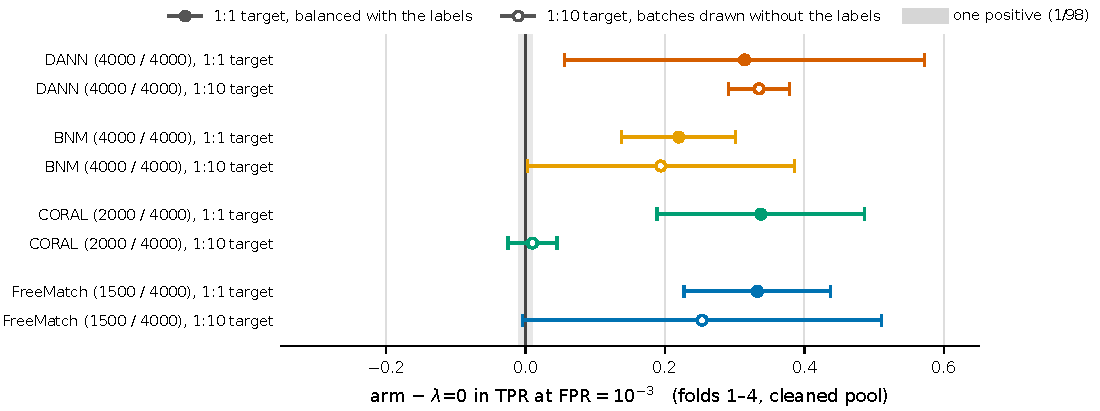
\includegraphics[width=0.92\textwidth]{F7_dilute10.pdf}
\caption{\textbf{The gain over the control with a 1:1 and a 1:10 target.} Per arm, the paired
$t$-interval of the balanced run minus the $\lambda=0$ control (filled) beside that of the
diluted run minus the same control, $G$ (open), folds 1--4, cleaned pool. Each arm is read at
its read-off step (DANN and BNM at \dlReadDann{}, CORAL at \dlReadCoral{}, FreeMatch at
\dlReadFm{}) and the control at 4000 in both. The control is shared: it was run once and is
reused for the 1:10 target, since no target gradient reaches its encoder or head; the target
enters only through the few half-precision steps it skips (Section~\ref{sec:arms}). The grey band is one
positive ($1/98$).}
\label{fig:dilute}
\end{figure}

\subsection{How far CORAL, DANN and FreeMatch can be ranked}
\label{sec:resolution}

At each arm's declared read-off, every paired interval among CORAL, DANN and FreeMatch includes
zero (Tables~\ref{tab:contrasts6} and~\ref{tab:k8pairs6}), so a single checkpoint per arm does
not rank them. Averaging each arm's scores over its last \rwFiveKWord{} checkpoints, the
pre-declared secondary analysis of Appendix~\ref{sec:failed}, FreeMatch has the highest
fold-mean under both score combinations. Its lead over DANN and CORAL excludes zero under the
secondary combination, mean rank, but not under the primary, mean logit
(Table~\ref{tab:k8pairs6}). We read this as a suggestive lead, not an established ranking: it
rests on the secondary combination, our intervals are probably too narrow
(Section~\ref{sec:intervals}), and these are further intervals without correction.

One point estimate per arm carries noise of its own: on a single run, the metric moves from one
checkpoint to the next even when nothing about the method changes. We measured this on the
stored checkpoints of the confirmatory folds. After removing each run's linear trend, the
per-fold scatter is $\rvSigmaMin{}$ to $\rvSigmaMax{}$, and consecutive checkpoints are close
to uncorrelated (lag-1 autocorrelation between $\rvLagMin{}$ and $\rvLagMax{}$). If the two
arms' checkpoint noise were independent, it alone would contribute $\rvNoiseMin{}$ to
$\rvNoiseMax{}$ to a difference of four-fold means; for at least one pair this exceeds the
standard error the paired interval implies, so arms trained on the same folds share much of
their checkpoint noise and the independent figure overstates it
(Appendix~\ref{sec:failed}, Figure~\ref{fig:resolution}). The benchmark likewise finds that, at
this sample size, which lenses are in the test set matters more than the model's
initialisation~\citep{lines2025simstosky}, and sampling theory gives the same direction for
validation sets of this size~\citep{oliver2018realistic}.

\subsection{Operating-point dependence and the benchmark ratio}
\label{sec:results-operating-point}

At 24\% purity the adaptation arms recover, as a share of the benchmark's completeness, CORAL
$\dLrCoral{}$\% $[\dLrCoralLo{}, \dLrCoralHi{}]$, FreeMatch $\dLrFreeMatch{}$\%
$[\dLrFreeMatchLo{}, \dLrFreeMatchHi{}]$, DANN $\dLrDann{}$\% $[\dLrDannLo{}, \dLrDannHi{}]$
and BNM $\dLrBnm{}$\% $[\dLrBnmLo{}, \dLrBnmHi{}]$; Appendix~\ref{app:perfold} gives the
completeness on each fold. One lens moves one fold's ratio by about \dlLensFoldPpWord{}
percentage points and the fold mean by about \dlLensMeanPpWord{} point; the intervals are wide
mainly because the folds differ. No arm's
fold-mean completeness reaches 0.50 at its declared read-off; DANN's sensitivity readout reaches
$\dLrDannSens{}$\%. The $\lambda=0$ control never reaches 24\% purity on two of its folds, so
it has no ratio. On the bright-only test pool, BNM's ratio falls from $\rvBnmDOneRatio{}$ to
$\rvBnmBrightRatio{}$ (Appendix~\ref{app:bright}).

The completeness--purity curves cross (Figure~\ref{fig:comppurity}). FreeMatch runs above
CORAL over $\dEightFmAbovePct{}$\% of the purity range and below it near 24\% purity, so a
single read at that line cannot rank them. AUROC, reported in the appendix tables, saturates:
the $\lambda=0$ control reaches $\dAuLambda{}$ in AUROC and $\dFmLambda{}$ at the operating
point. An unadapted lens finder elsewhere reached an AUROC of 0.921 with a TPR of zero at
FPR${}=0.1\%$~\citep{parul2024}.

\begin{figure}[t]
\centering
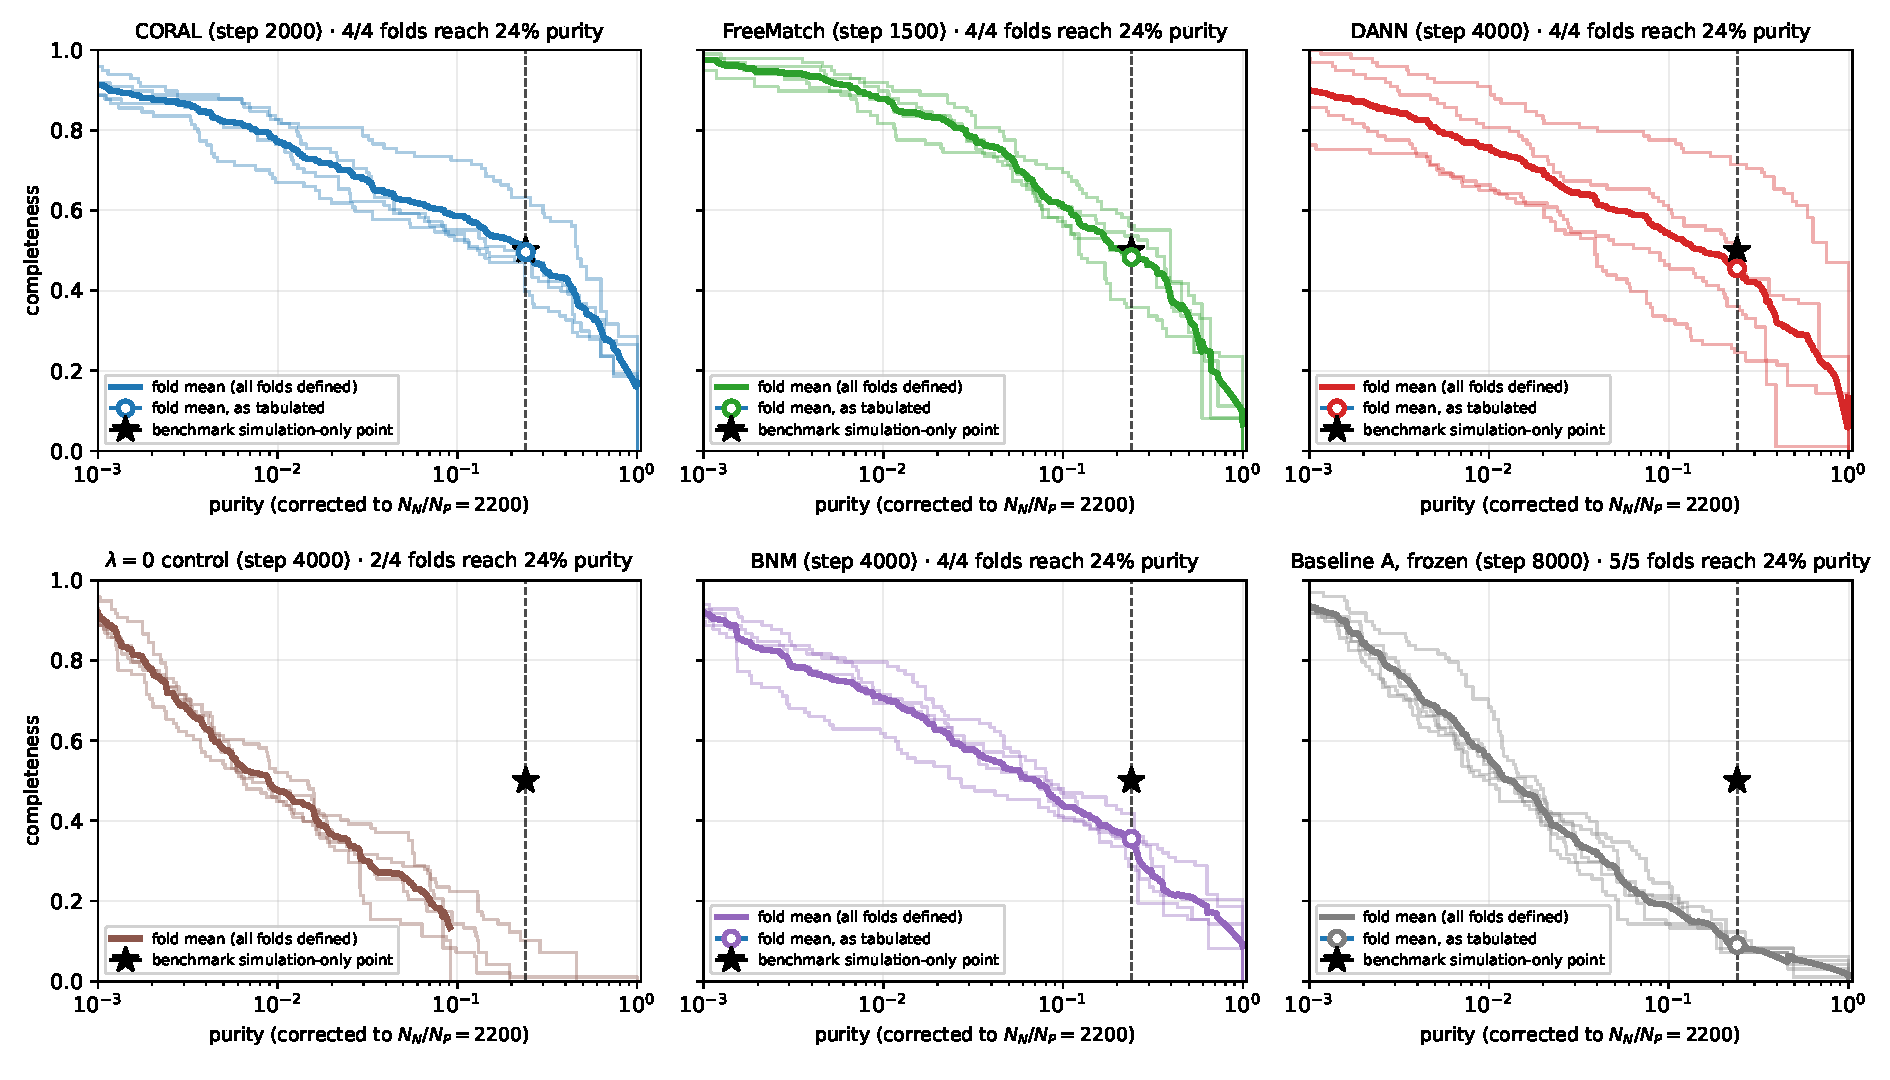
\includegraphics[width=\textwidth]{F6_completeness_purity_v2.pdf}
\caption{\textbf{Completeness against prevalence-corrected purity}, one panel per arm, at the
arm's read-off step; a secondary readout beside the primary TPR@$10^{-3}$. Thin lines are
folds, the thick line the fold mean where every fold is defined, the open circle the tabulated
fold mean, the dashed line 24\% purity and the star the benchmark's simulation-only operating
point. Each panel title gives how many folds reach 24\% purity; a curve that stops before the
dashed line is a fold that never reaches it.}
\label{fig:comppurity}
\end{figure}

\subsection{What the models find and miss}
\label{sec:findmiss}

Every model recovers grade-A lenses about two to three times
($\rvGradeRatioMin{}$ to $\rvGradeRatioMax{}$) as often as grade-B lenses
(Table~\ref{tab:graderecall}). Recall rises with the expert score in every model, and for the
adaptation arms it is lowest for the smallest Einstein radii (Appendix~\ref{app:breakdowns});
modelled Einstein radii exist for $\rvThetaN{}$ of the $\rvConfTestN{}$ confirmatory test
lenses. The lenses that all six models miss (the four adaptation arms, Baseline A and the
control) are mostly grade B ($\rvMissedAllB{}$ of
$\rvMissedAllN{}$), and in the gallery they tend to have small or faint arcs or unusual
configurations (Figure~\ref{fig:gallery}).

The highest-scoring negatives are mostly bright, compact galaxies with extended halos, face-on
spirals, and galaxies with rings or arc-like arms, which are familiar false positives for lens
finders. Of the $\rvTopNegN{}$ negatives that score in the top 30 of any of the seven readouts on any fold,
$\rvTopNegC{}$ are graded C in the Discovery Engine catalogue, the grade below the A and B
cuts that define our positives; none is grade A, B or X. We list the most frequently high-scoring
negatives in Appendix~\ref{app:breakdowns} for inspection and make no claim about their
nature. The \rwAboveN{} negatives above threshold in any cell are brighter than the pool as a
whole: $\rvAboveFaintPct{}$\% are fainter than $I_E = 22.5$, against $\rvPoolFaintPct{}$\% of
all test negatives. Restricting the test negatives to objects brighter than 22.5, the
benchmark's depth, leaves every contrast we recomputed (Table~\ref{tab:bright}) with the same
zero-inclusion (Appendix~\ref{app:bright}).

% GENERATED FILE -- do not edit by hand.
% Rebuild:  python make_all.py (generator: make_main_tables_v2.py)
% Table (rewrite v1): recall by grade, from audit/review_r1/out/A3_recall_by_grade.json.
\begin{table}[tbp]
\centering
\caption{\textbf{Recall by grade} at each fold's FPR${}=10^{-3}$ threshold on the cleaned pool, summed over folds 1--4: recovered/total, rate, and Clopper--Pearson 95\% interval. Descriptive only; no contrast is formed. Per-fold counts: Appendix~\ref{app:breakdowns}.}
\label{tab:graderecall}
\footnotesize
\setlength{\tabcolsep}{4pt}
\begin{tabular}{lrrrrrr}
\toprule
 & \multicolumn{3}{c}{grade A} & \multicolumn{3}{c}{grade B} \\
\cmidrule(lr){2-4}\cmidrule(lr){5-7}
Readout & found & rate & 95\% CI & found & rate & 95\% CI \\
\midrule
Baseline A & 52/196 & $0.27$ & $[0.20, 0.33]$ & 20/195 & $0.10$ & $[0.06, 0.15]$ \\
$\lambda=0$ control & 55/196 & $0.28$ & $[0.22, 0.35]$ & 17/195 & $0.09$ & $[0.05, 0.14]$ \\
BNM & 116/196 & $0.59$ & $[0.52, 0.66]$ & 42/195 & $0.22$ & $[0.16, 0.28]$ \\
FreeMatch & 136/196 & $0.69$ & $[0.62, 0.76]$ & 66/195 & $0.34$ & $[0.27, 0.41]$ \\
DANN & 129/196 & $0.66$ & $[0.59, 0.72]$ & 66/195 & $0.34$ & $[0.27, 0.41]$ \\
DANN, 2000 & 144/196 & $0.73$ & $[0.67, 0.80]$ & 73/195 & $0.37$ & $[0.31, 0.45]$ \\
CORAL & 139/196 & $0.71$ & $[0.64, 0.77]$ & 65/195 & $0.33$ & $[0.27, 0.40]$ \\
\bottomrule
\end{tabular}
\end{table}


\begin{figure}[t]
\centering
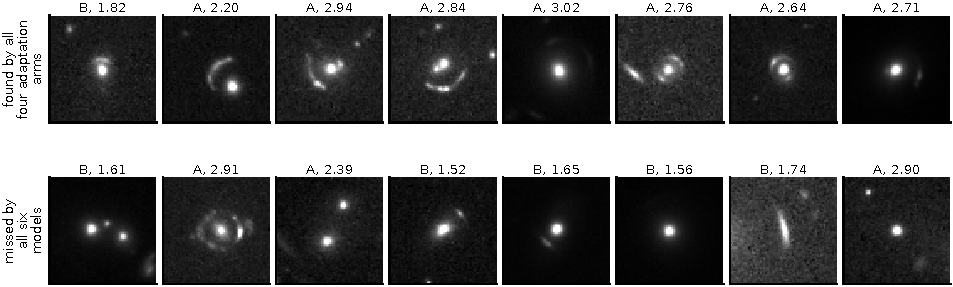
\includegraphics[width=\textwidth]{FY_lens_gallery.pdf}
\caption{\textbf{Confirmatory test lenses found and missed.} Top: the first eight, by Euclid
ID, recovered by all four adaptation arms; bottom: the first eight missed by all six models
(the four adaptation arms, Baseline A and the control). Each
panel gives the grade and expert score, under the encoder's input stretch. Image credit: ESA
Euclid/Euclid Consortium/NASA/Q1-2025.}
\label{fig:gallery}
\end{figure}
